\documentclass[11pt,a4paper]{article}
\usepackage[utf8]{inputenc}
\usepackage{mathtools}
\usepackage[norsk]{babel}
\usepackage{graphicx}
\usepackage{gensymb}

\usepackage{listings}
\usepackage{color}
 
\definecolor{dkgreen}{rgb}{0,0.6,0}
\definecolor{gray}{rgb}{0.5,0.5,0.5}
\definecolor{mauve}{rgb}{0.58,0,0.82}


\lstset{ %
  language=sql,                % the language of the code
  basicstyle=\small,           % the size of the fonts that are used for the code
  numbers=left,                   % where to put the line-numbers
  numberstyle=\small\color{gray},  % the style that is used for the line-numbers
  stepnumber=1,                   % the step between two line-numbers. If it's 1, each line 
                                  % will be numbered
  numbersep=5pt,                  % how far the line-numbers are from the code
  backgroundcolor=\color{white},      % choose the background color. You must add \usepackage{color}
  showspaces=false,               % show spaces adding particular underscores
  showstringspaces=false,         % underline spaces within strings
  showtabs=false,                 % show tabs within strings adding particular underscores
  frame=none,                   % adds a frame around the code
  rulecolor=\color{black},        % if not set, the frame-color may be changed on line-breaks within not-black text (e.g. commens (green here))
  tabsize=2,                      % sets default tabsize to 2 spaces
  captionpos=b,                   % sets the caption-position to bottom
  breaklines=true,                % sets automatic line breaking
  breakatwhitespace=false,        % sets if automatic breaks should only happen at whitespace
  title=\lstname,                   % show the filename of files included with \lstinputlisting;
                                  % also try caption instead of title
  keywordstyle=\color{blue},          % keyword style
  commentstyle=\color{dkgreen},       % comment style
  stringstyle=\color{mauve},         % string literal style
  escapeinside={\%*}{*)},            % if you want to add LaTeX within your code
  morekeywords={*,...}               % if you want to add more keywords to the set
}

\title{Notater: INF1300}
\author{Veronika Heimsbakk \\ 
veronahe@student.matnat.uio.no}
\begin{document}

\maketitle{}
\tableofcontents
\newpage{}

\section{ORM}
\subsection{Setningers aritet}
Den elementære setningen \textit{Studenten med navn Anne fikk i emned med emnekode INF1010 resultatet karakteren B} inneholder tre begreper: \textit{student}, \textit{emne} of \textit{resultat}. Antall begreper i en setningen kalles setningens aritet. Vårt eksempel har aritet 3. 

\begin{itemize}
\item{Setninger med aritet 1 kaller vi unære.}
\item{Setninger med aritet 2 kaller vi binære.}
\item{Setninger med aritet 3 kaller vi ternære.}
\end{itemize}

Setninger med aritet større enn 3 er sjeldne.

\subsection{Faktatyper og broer i ORM}
\begin{figure}[h!]
	\centering
		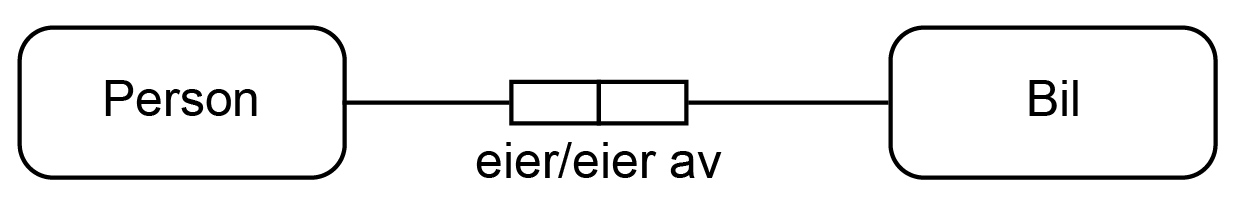
\includegraphics[width=200px]{img/fakta-01.png}
	\caption{Et eksempel på faktatype mellom begrepen Person og Bil.}
\end{figure}

En \textbf{bro} er en forbindelse mellom et begrep og en representasjon.
\begin{figure}[h!]
	\centering
		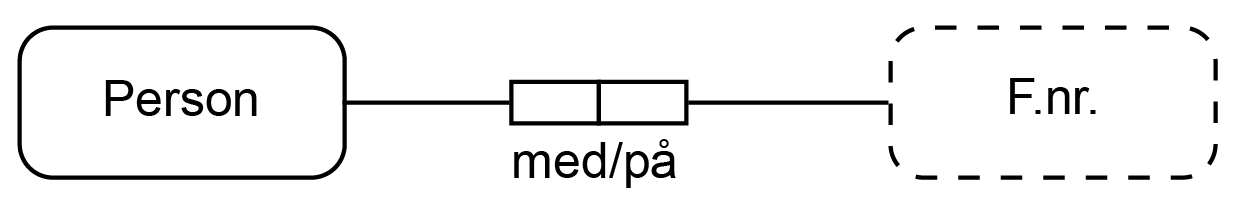
\includegraphics[width=200px]{img/bro-01.png}
	\caption{Et eksempel på en bro.}
\end{figure}

\textbf{Setningstyper} er en fellesbetegnelse på faktatyper og broer. Broer er alltid binære, faktatyper kan ha vilkårlig antall roller (aritet).
I faktatyper bør alle rollenavn inneholde er verb. I alle broer er det vanlig med preposisjoner som rollenavn. De to vanligste rolleparene er \textbf{med/for} og \textbf{med/på}.

\subsection{Forekomsttabeller og entydighetsskranker}
\begin{figure}[h!]
	\centering
		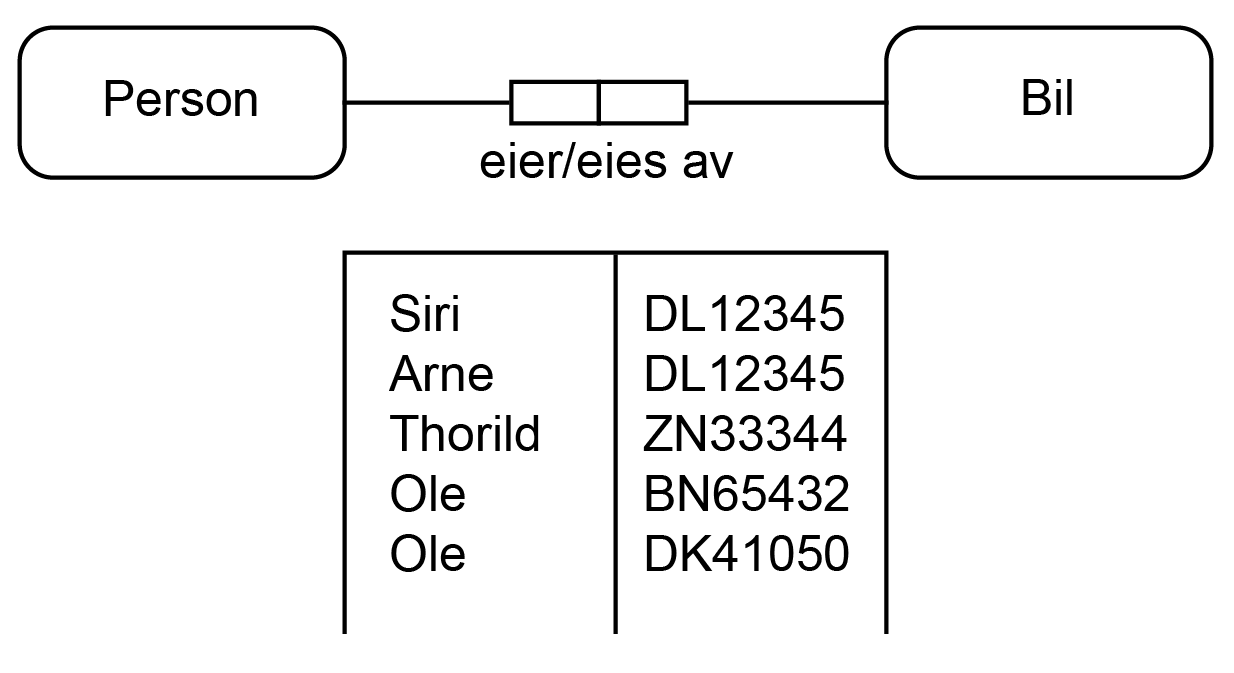
\includegraphics[width=200px]{img/for-01.png}
	\caption{Eksempel på forekomsttabell.}
\end{figure}

\begin{figure}[h!]
	\centering
		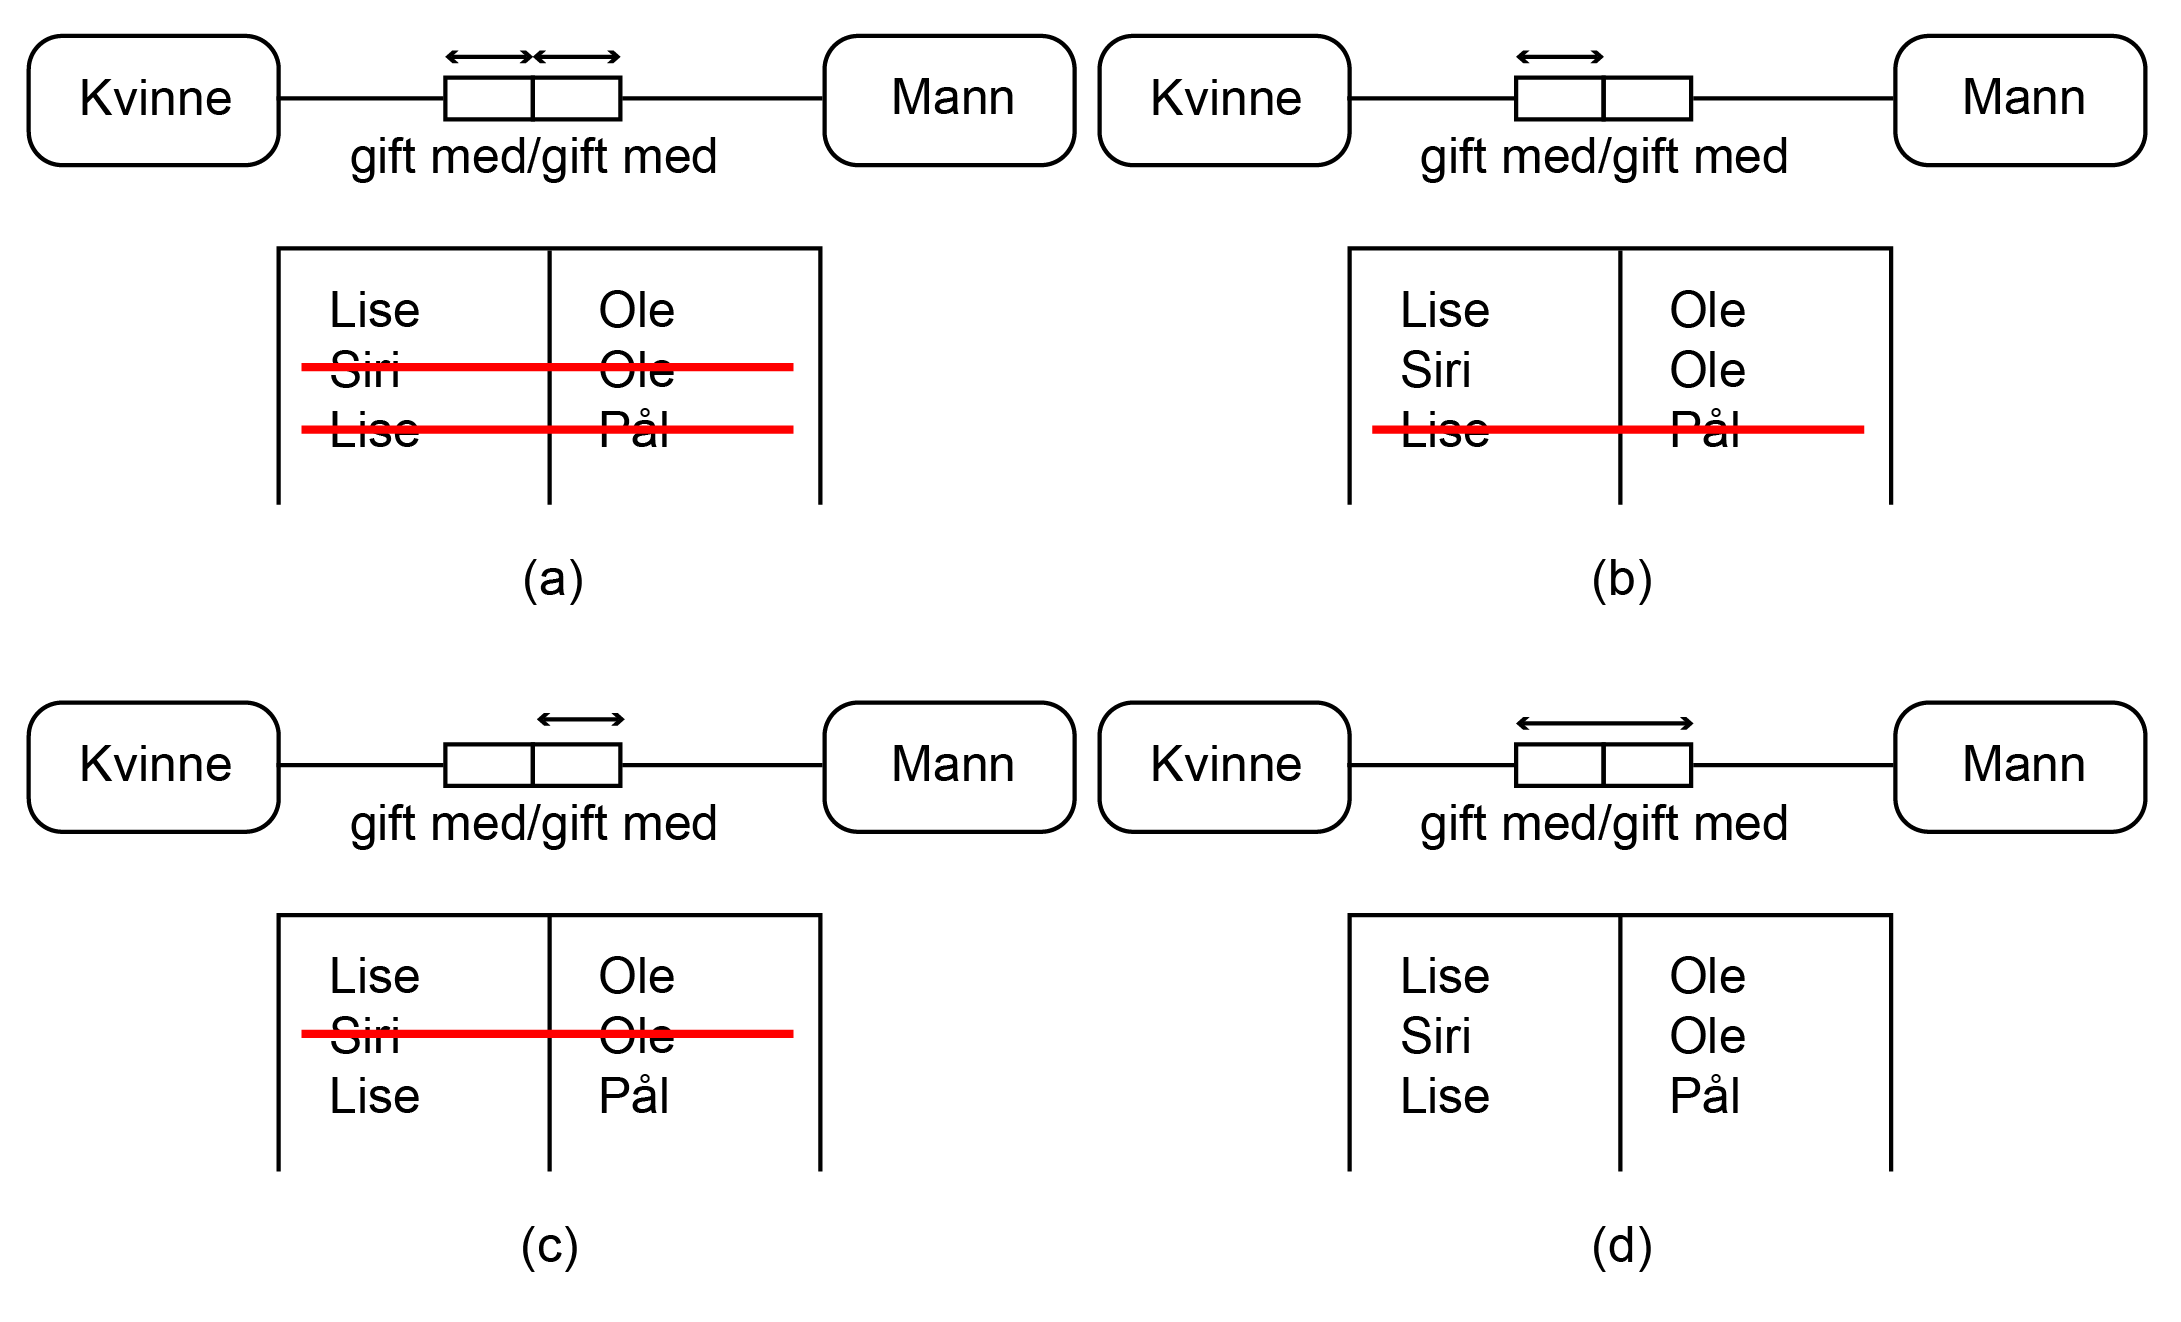
\includegraphics[width=\linewidth]{img/sk-01.png}
	\caption{Eksempel på entydighetsskranker.}
\end{figure}

I Fig. 4(a) er Norges eneste lovlige ekteskapsform, denne kalles 1:1 (én-til-én) faktatype mellom (bekrepene) Kvinne og Mann.
I Fig. 4(b) har vi flerkoneri, dette er n:1 (mange-til-én).
I Fig. 4(c) har vi flermanneri, dette er 1:n (én-til-mange).
I Fig. 4(d) har vi flergifte, dette er m:n (mange-til-mange) faktatype.

\subsection{Totale roller og perfekte broer}
\begin{figure}[h!]
	\centering
		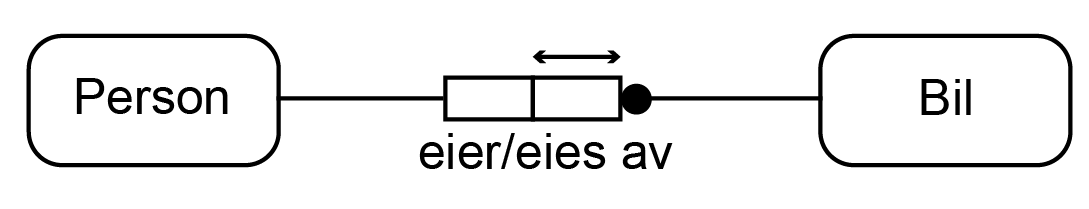
\includegraphics[width=200px]{img/tot-01.png}
	\caption{Eksempel på en total rolle.}
\end{figure}

Dersom alle biler har en eier, sier man at vi har en total funksjon fra Bil til Person (den er definert for alle forekomster av Bil).
Vi sier at rollen \textit{eies av} er en \textbf{total rolle} for Bil og markerer det med en kule (liten fylt sirkel) på rollen. 

\begin{figure}[h!]
	\centering
		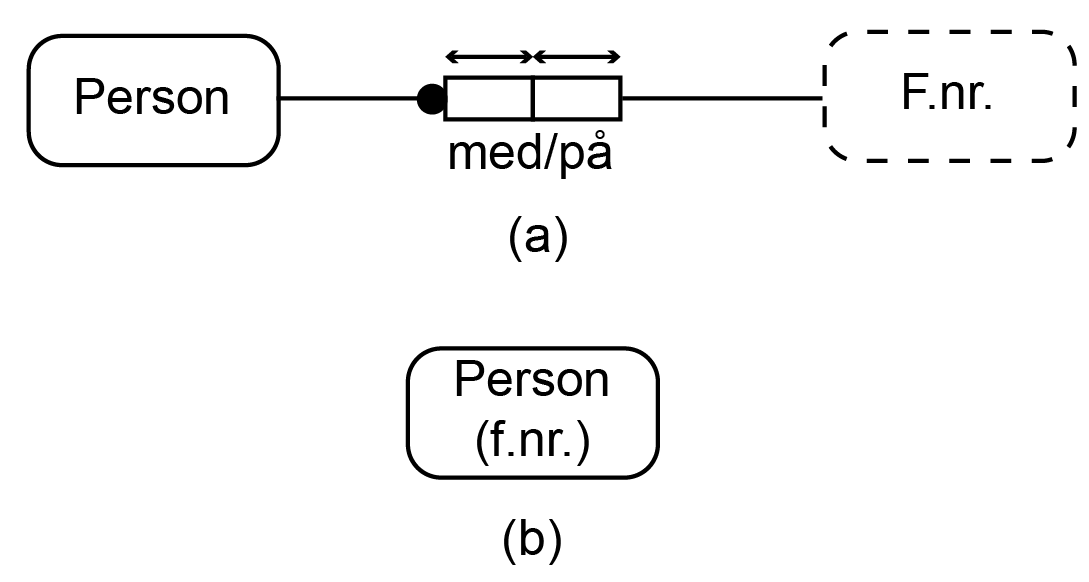
\includegraphics[width=200px]{img/perf-01.png}
	\caption{Eksempel på en perfekt bro.}
\end{figure}

En 1:1 bro der begrepsrollen er total, kalles en \textbf{perfekt bro}. Perfekte broer (Fig. 5(a)) er så vanlige at vi har en egen kortform for dem, vist i Fig. 5(b). De to tegnemåtene er ekvivalente.

\subsection{Begrepsdannelse}
Setning: \textit{På Bildern klokken 8 målte Jens 9 grader.} Her er \textit{Blindern} et \textbf{sted} med representasjon \textbf{stedsnavn}. \textit{8} er et \textbf{tidspunkt} med representasjon \textbf{dato og klokkeslett}. \textit{Jens} er en \textbf{person} med representasjon \textbf{personnavn}. \textit{9} er en \textbf{temperatur} med representasjon \textbf{\celsius}

\begin{figure}[h!]
	\centering
		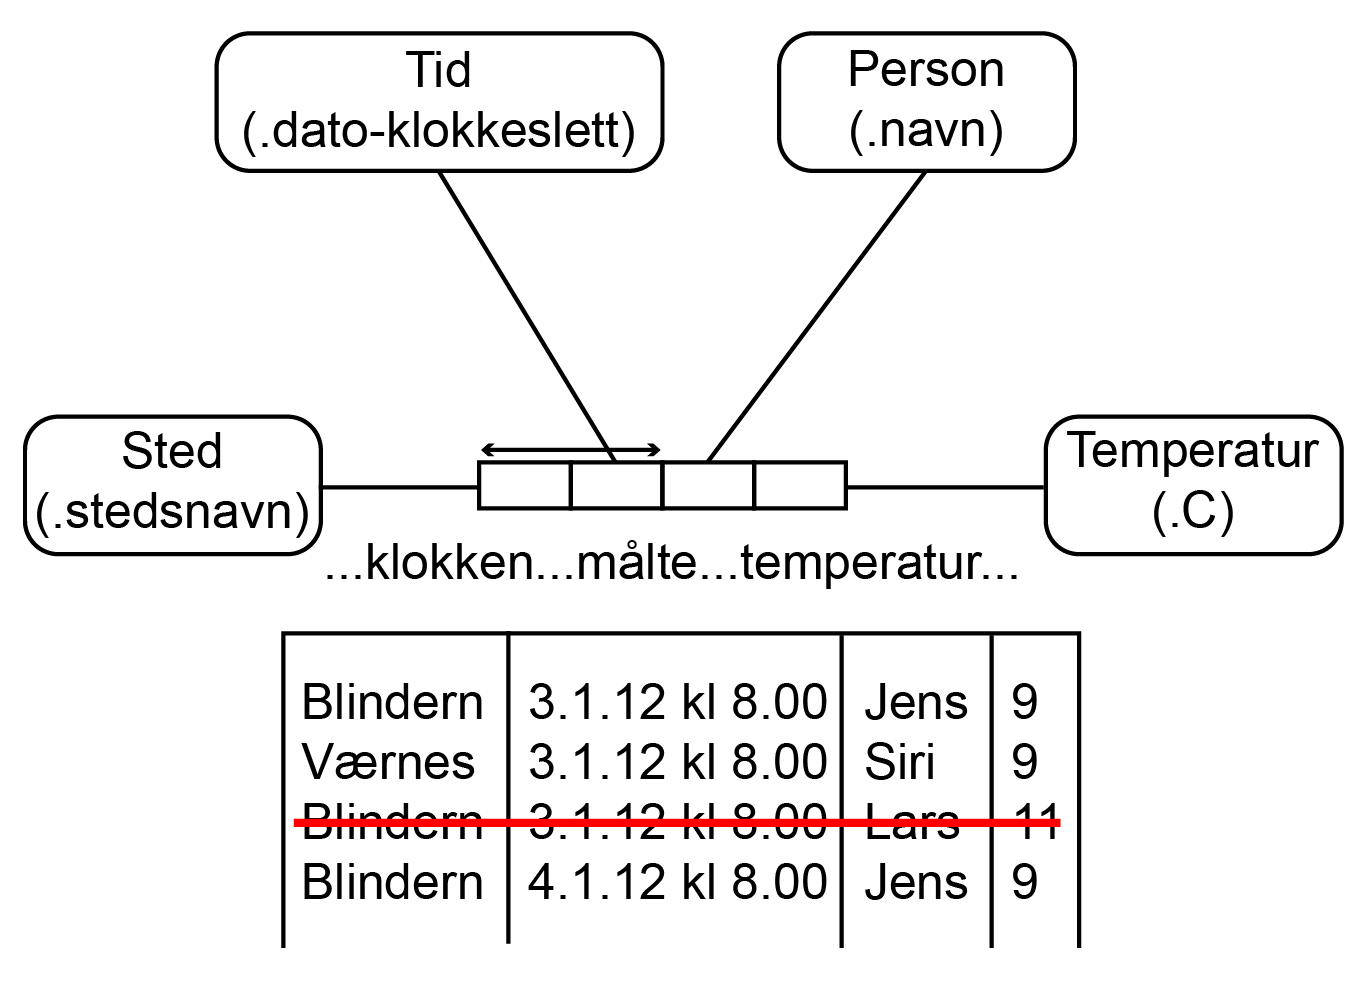
\includegraphics[width=300px]{img/2-01.png}
	\caption{Eksempel på begrepsdannelse.}
\end{figure}

\begin{figure}[h!]
	\centering
		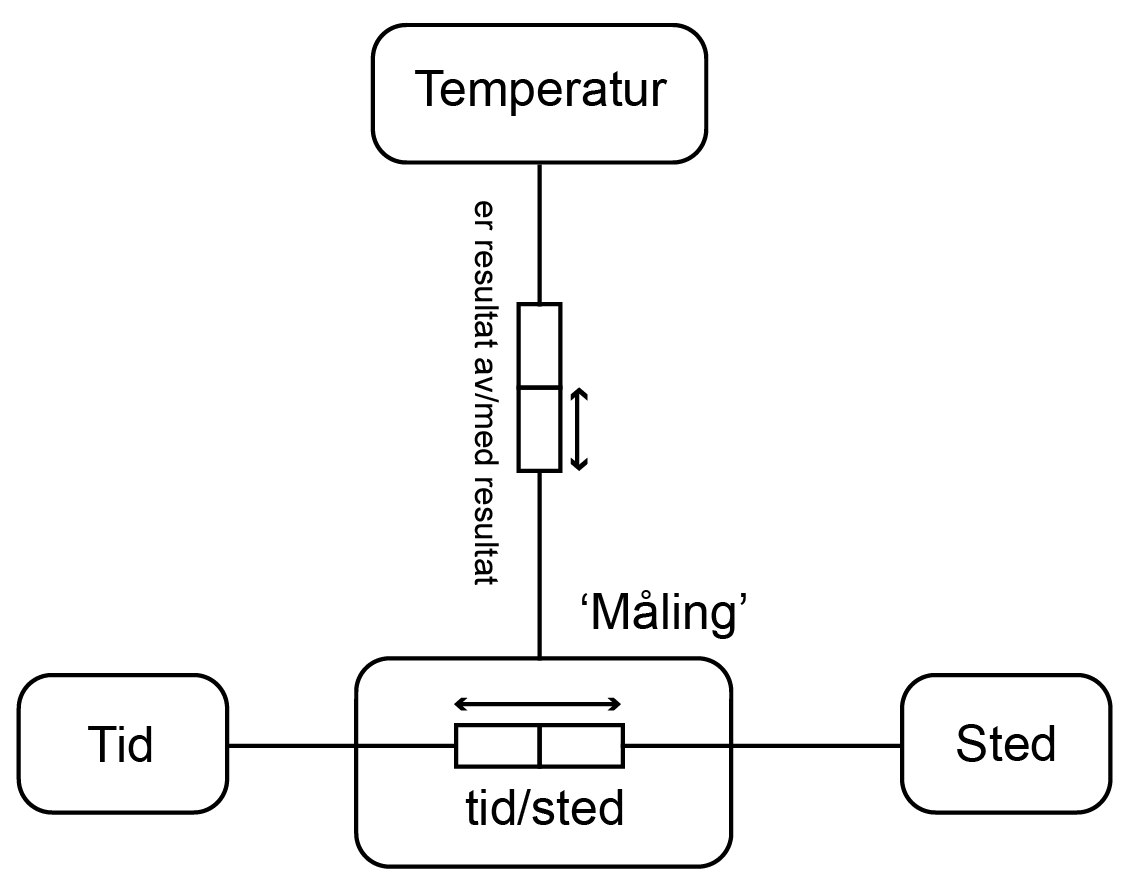
\includegraphics[width=250px]{img/alt-01.png}
	\caption{Alternativ notasjon.}
\end{figure}

\subsection{Ekstern entydighetsskranke}
\begin{figure}[h!]
	\centering
		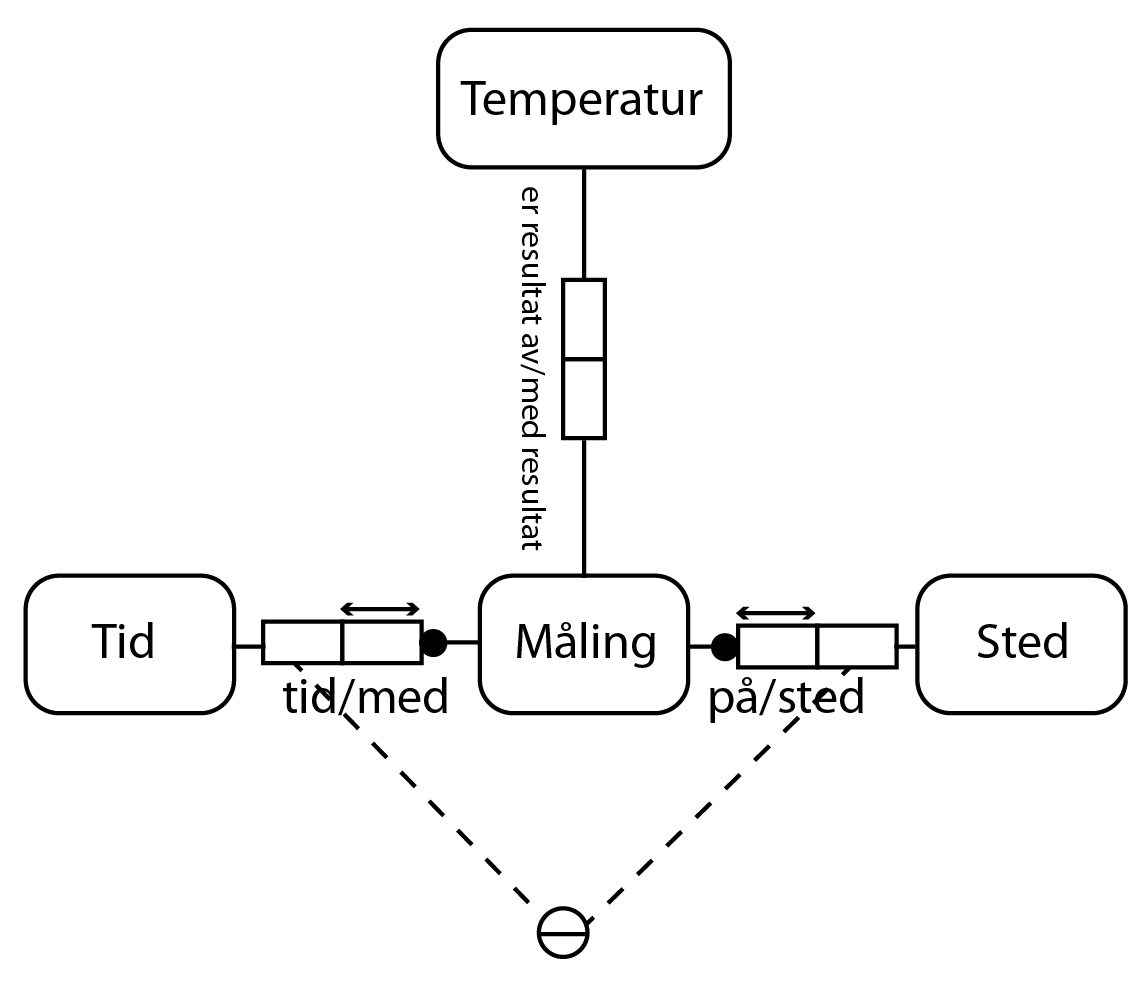
\includegraphics[width=250px]{img/ents-01.png}
	\caption{Eksempel på en ekstern endydighetsskranke.}
\end{figure}

Entydighet på tvers av faktatyper indikerer vi med en \textbf{ekstern entydighetsskranke} på de involverte rollene \textit{tid} og \textit{sted}. Fig. 9.

\begin{figure}[h!]
	\centering
		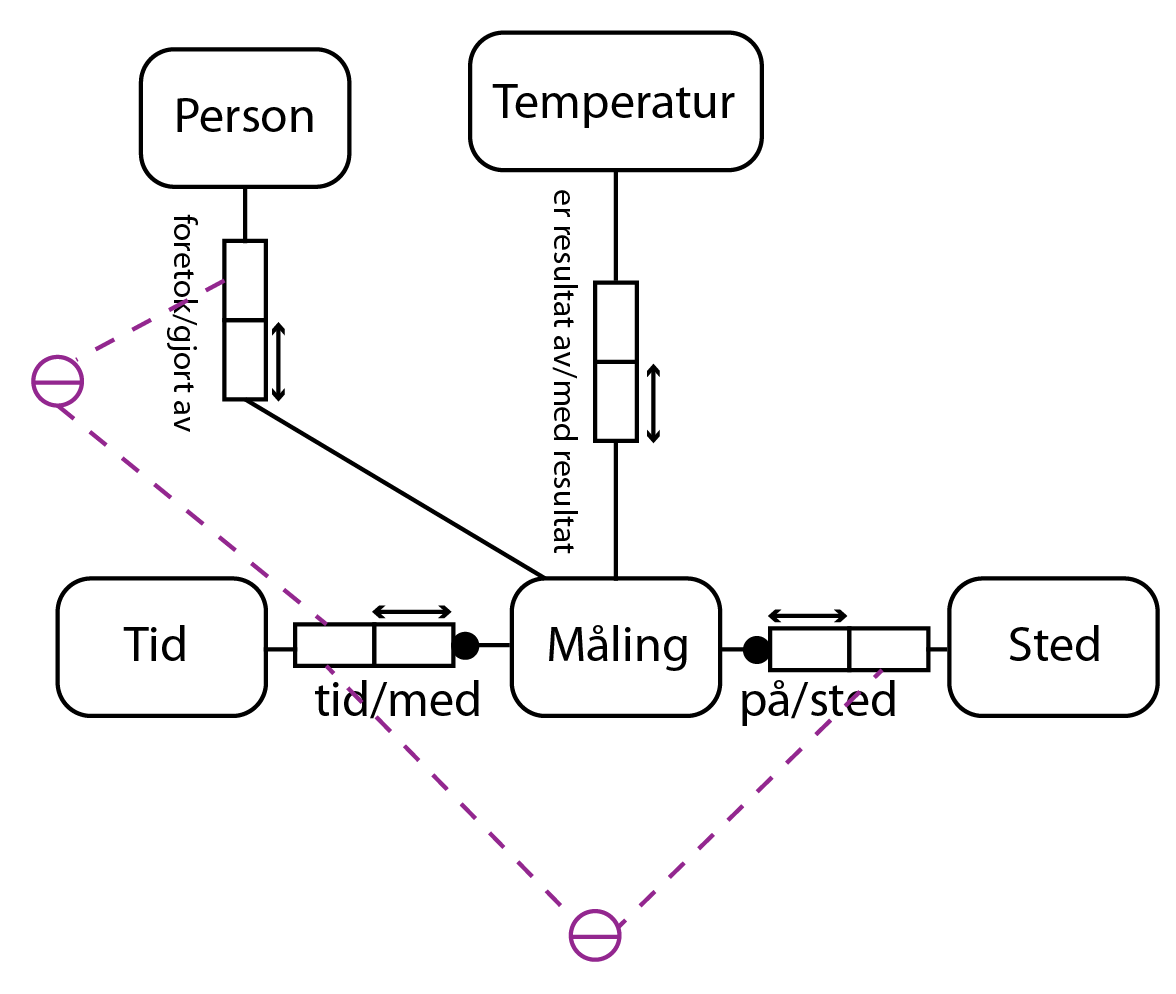
\includegraphics[width=250px]{img/ents2-01.png}
	\caption{Eksempel på en ekstern endydighetsskranke.}
\end{figure}

I Fig. 10, uttrykker vi at en person ikke kan foreta mer enn én måling av gangen. Dette gjøres med en ekstern entydighetsskranke på rollene \textit{foretok} og \textit{tid}.

Alle entydighetsskranker som går over mer enn én rolle i en faktatype, skjuøer et (nytt) begrep. Man skal alltid vurdere om det skal lages nye begreper når man får faktatyper med lange entydighetspiler. En faktatype med aritet 3 eller 4 (eller mer) kan gjøres om til binære setninger ved å lage ett eller flere nye begreper. Eksempelsvis har Fig. 7 aritet 4.

\subsection{Populasjoner}
\paragraph{Populasjon for en rolle}
Hvis $r$ er en rolle, betegner \textbf{pop(r)} mengden av forekomster i kolonnen for $r$ i forekomsttabellen.

\paragraph{Populasjon for et begrep}
Begreper har egentlig ikke forekomster løsrevet fra roller, men vi definerer likevel populasjonen til et begrep $A$ som har roller $r_1, r_2, \dots, r_n$ ved $pop(A) = pop(r_1) \cup pop(r_2) \cup \dots \cup pop(r_n)$

\textbf{Merk}: populasjonen til en rolle/et begrep varierer med tiden.

\subsection{Mengdeskranker}
Mengdeskrankene begrenser mengden av forekomster i en eller flere roller i forhold til forekomstene i andre roller. Det finnes følgende varienter: 
\begin{itemize}
\item{Likhetsskranke}
\item{Ulikhetsskranke}
\item{Delmengdeskranke}
\end{itemize}

\subsubsection{Mengdeliketsskranke}

\begin{figure}[h!]
	\centering
		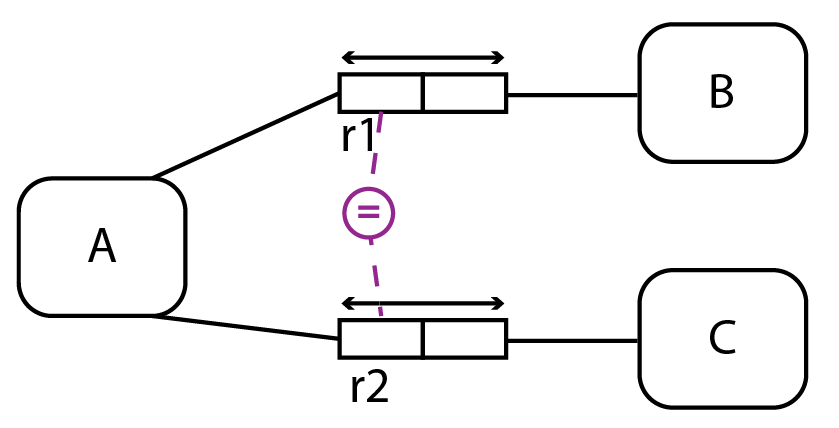
\includegraphics[width=150px]{img/men-01.png}
	\caption{Eksempel på en ekstern mengdelikhetsskranke.}
\end{figure}

$A$ skal ha rollen $r1$, hvis og bare hvis, $A$ har rollen $r2$. 
$pop(r1) = pop(r2)$ for alle tilstander.

\subsubsection{Mengdeulikhetsskranke}

\begin{figure}[h!]
	\centering
		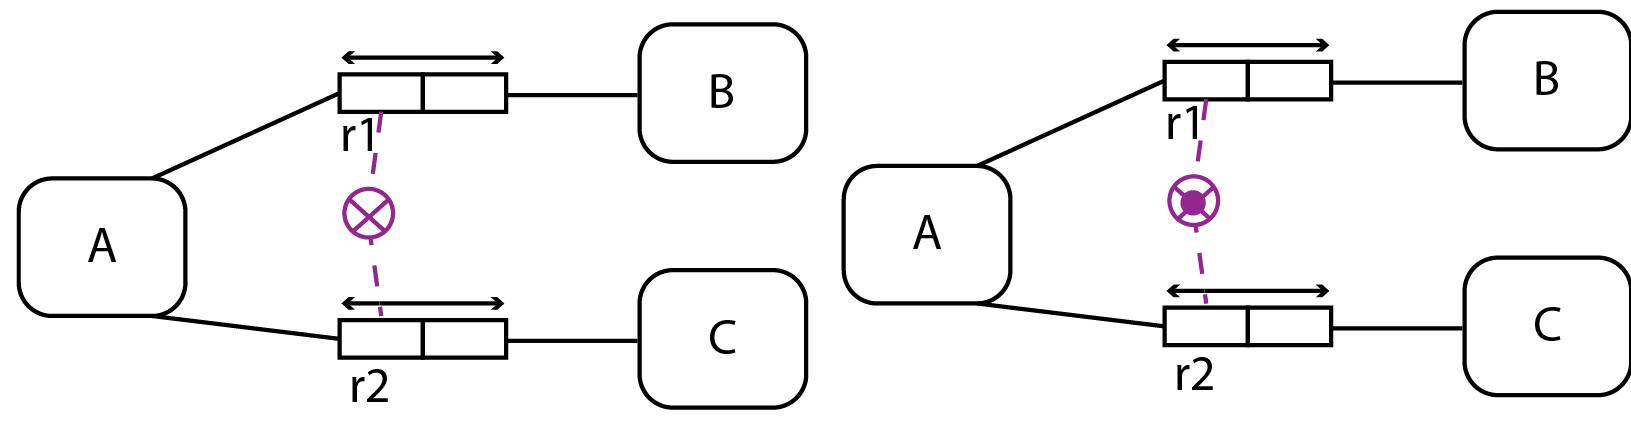
\includegraphics[width=300px]{img/menu2-01.png}
	\caption{Eksempel på en ekstern mengdeulikhetsskranke.}
\end{figure}

$A$ skal ikke ha både rollen $r1$ og $r2$.
$pop(r1) \cap pop(r2) = \emptyset $

I den andre figuren i Fig. 12, skal $A$ ha en og bare en av rolle $r1$ og $r2$.

\subsubsection{Delmengdeskranke}

\begin{figure}[h!]
	\centering
		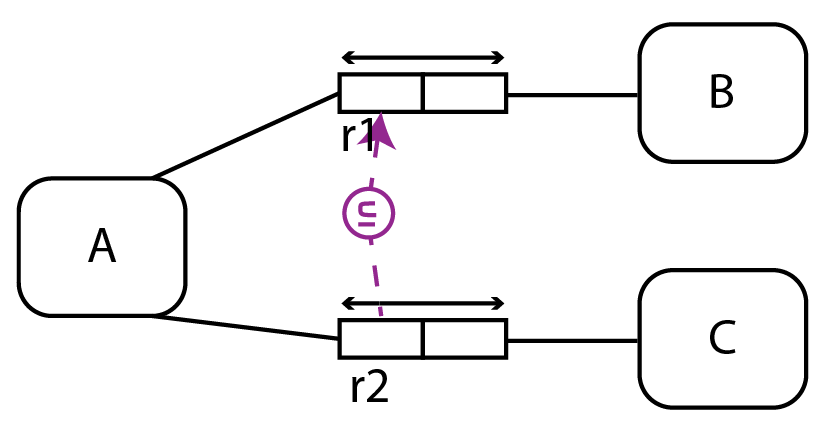
\includegraphics[width=150px]{img/delm-01.png}
	\caption{Eksempel på en ekstern delmengdeskranke.}
\end{figure}

Hvis $A$ har rollen $r2$, så skal $A$ også ha rollen $r1$.
$pop(r2) \subseteq pop(r1)$ for alle tilstander.

\subsection{Underbegreper}
Kan alle tenkelige forekomster av et begrep spille alle roller som er knyttet til begrepet? Hvis nei, kan vi få en mer presis modell ved å innføre \textbf{underbegreper}.

$B$ er et underbegrep av $A$ hvis vi alltid har at $pop(B) \subseteq pop(A)$.
\begin{figure}[h!]
	\centering
		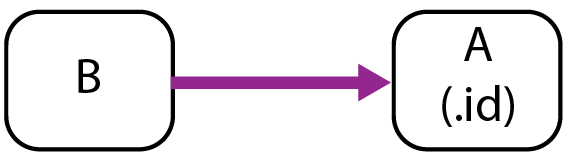
\includegraphics[width=150px]{img/und-01.png}
	\caption{Notasjon: underbegreper.}
\end{figure}

Underbegreper arver representasjon og roller fra superbegrepet. I tillegg har de sine egne roller. Underbegrepsskranker brukes til å bestemme hvilket underbegrep hver enkelt forekomst tilhører. De kan overlappe eller være disjunkte. Underbegreper kan, men må ikke, være uttømmende mhp. sitt superbegrep. Resonnementer over entydighetsskranker, totale rolle og underbegrepsskrankene avslører om underbegrepene er overlappende og/eller uttømmende.

\begin{figure}[h!]
	\centering
		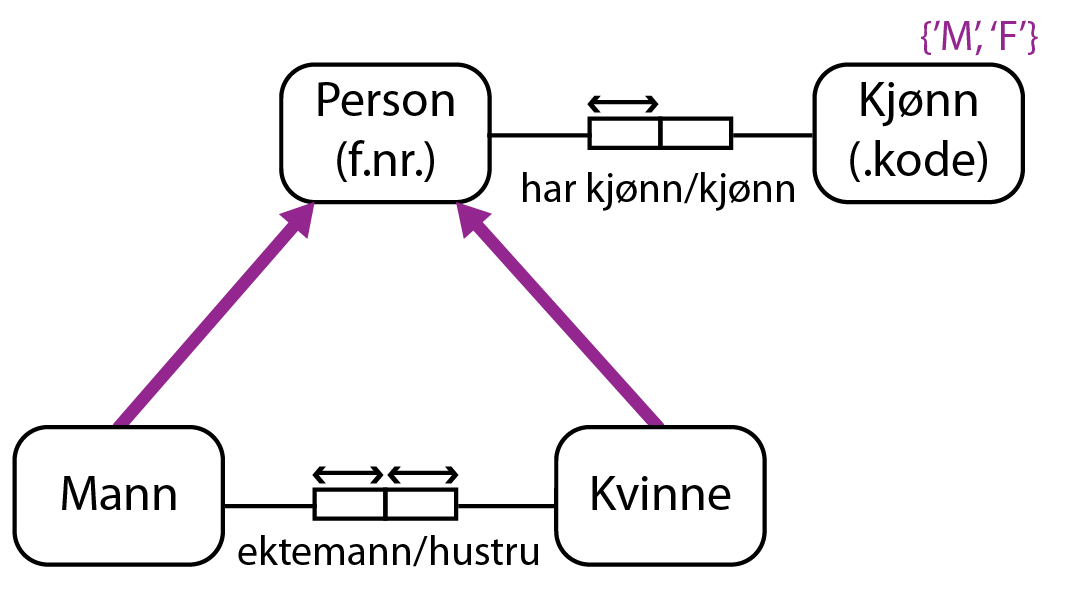
\includegraphics[width=200px]{img/undeks-01.png}
	\caption{Eksempel med underbegrepsskranke. Hver Mann er en Person som har \textit{kjønn} 'M'. Hver Kvinne er en Person som har \textit{kjønn} 'F'.}
\end{figure}

\subsection{Kombinert total rolle}
\begin{figure}[h!]
	\centering
		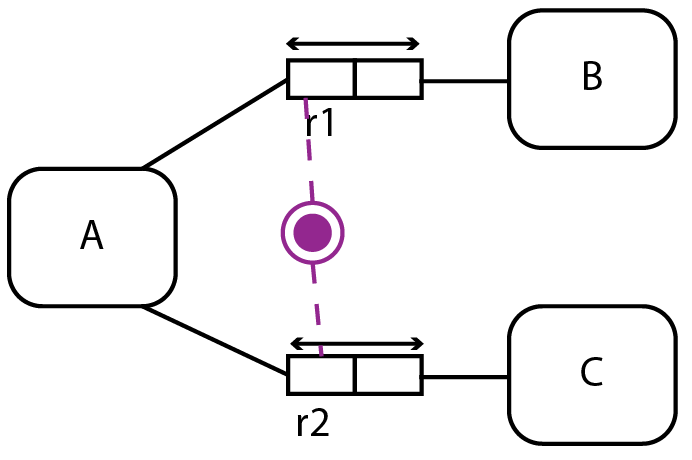
\includegraphics[width=150px]{img/ktot-01.png}
	\caption{Kombinert total rolle.}
\end{figure}

$A$ skal ha enten rollen $r1$ eller rollen $r2$. $pop(r1) \cup pop(r2) = pop(A)$ for alle tilstander.

\section{SQL}

\subsection{Nøkler og nøkkelatributter}
\begin{figure}[h!]
	\centering
		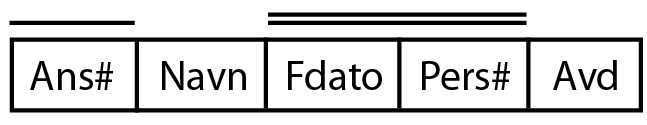
\includegraphics[width=150px]{img/nok-01.png}
	\caption{To ansatte skal ikke kunne ha samme Ans\# og to personer kan aldri ha samme fødselsnummer.}
\end{figure}

Primærnøkler blir markert med én strek. Andre kandidatnøkler er i dette tilfellet markert med to streker. 

\subsubsection{Fremmednøkler}
Fremmednøkler må ha samme antall attributter som primærnøkkelen i den relasjonen den peker ut, og attributtene må ha parvis samme domener. (Noen databasesystemer tillater også fremmednøkler til kandidatnøkler som ikke er primærnøkler.)
Korresponserende attributter behøver ikke å ha samme navn. Det er lov å ha fremmednøkler til «seg selv». Fremmednøkler benyttes til å uttrykke integritetsregler.

\paragraph{Påkrevde integritetsregler i relasjonsdatabaser}
\begin{itemize}
\item{\textbf{Entitetsintegritet:} Alle relasjonsskjemaer skal ha en og bare en primærnøkkel. Ingen av attributtene i en primærnøkkel får være \textbf{null}.}
\item{\textbf{Referanseintegritet:} Hvis fremmednøkkelen ikke er \textbf{null}, så skal det finnes et tuppel i den refererte relasjonen hvor primærnøkkelen har samme verdi som fremmednøkkelen (dvs. at det refererte tuppelet skal eksistere).}
\end{itemize}

\subsection{create table}
\lstinputlisting{code/create.sql}

Ansatte skal ikke kunne ha samme AId, to personer kan aldri ha samme fødselsnummer = Fdato + Pnr. Dermed er både AId of (Fdato, Pnr) kandidatnøkler. Vi velger AId som primærnøkkel og markerer (Fdato, Pnr) som kandidatnøkkel.

Maks en primærnøkkeldeklarasjon pr. relasjon. Kandidatnøkler kan deklareres i \texttt{create table} sammen med nøkkelattributtet med \texttt{unique}.

\subsection{Skranke på ett attributt}
\lstinputlisting{code/notnull.sql}
Kan ikke sette inn tuppel med verdien null i dette attributtet. Kan ikke endre verdien til null senere.

\lstinputlisting{code/check.sql}
Angir en betingelse på attributtet. Sjekkes ved hver endring av attributtets verdi.

\subsection{select}
\lstinputlisting{code/select.sql}
Svar på oppgaven: finn navn og startdato for alle prosjekter bestilt av kunden «Pust og pes AS». Sorter dem slik at det nyeste prosjektet kommer først.

\subsection{Tekstmønstre}
\lstinputlisting{code/tekst.sql}
\texttt{\_} passer med \textit{ett} vilkårlig tegn, og \texttt{\%} passer med en vilkårlig tekststring (flere enn ett tegn).

\lstinputlisting{code/tekst2.sql}
Her blir resultatet en tabell over navn og kjønn på personer som har akkurat tre tegn i fornavn og et etternavn som ikke slutter på \textit{sen}.

\subsection{Aggregeringsfunksjoner}
\begin{table}[h!]
\begin{center}
\begin{tabular}{| l | l |}
\hline
\textbf{navn} & \textbf{virkning} \\
\hline
count & teller antall \\
\hline
min & finner minste verdi \\
\hline
max & finner største verdi \\
\hline
sum & summerer verdier \\
\hline
avg & finner snittet av verdier \\
\hline
\end{tabular}
\end{center}
\caption{Aggregeringsfunksjoner.}
\end{table}

\subsubsection{count()}
\lstinputlisting{code/count.sql}
\begin{enumerate}
\item{Gir antall tupler i tabellen.}
\item{Som for alle attributter i select-listen, kan vi gi \texttt{count(*)} et nytt navn.}
\item{Gir antall tupler i tabellen hvor attributtet \texttt{gender} ikke er null.}
\item{Gir antall forskjellige verdier i attributtet \texttt{firstname} (null telles ikke med).}
\end{enumerate}

\subsubsection{min() og max()}
\lstinputlisting{code/minmax.sql}
Ved tabellen \texttt{ansatt(anr, navn, lonn, avd)}, så finner vi her den største lønnsforskjellen ved Ifi.
Det er ikke lov å ha regneuttrykk som parameter i \texttt{min()} og \texttt{max()}.

\subsubsection{sum() og avg()}
\lstinputlisting{code/sumavg.sql}
Ved tabellen \texttt{ansatt(anr, navn, lonn, avd)}, så finner vi her summen av lønnsutgifter og gjennomsnittslønn for Ifi.

\subsubsection{Et eksempel}
Gitt tabellen \texttt{ansatt(anr, navn, lonn, avd)}, finn antall ansatte ved Ifi som tjener mer enn det dobbelte av snittlønna i administasjonen.
\lstinputlisting{code/eks1.sql}
\textit{Merk:} en \texttt{select} inne i en \texttt{where}-betingelse må være omsluttet av parenteser.

\subsubsection{group by}
Finn antall ansatte i hver avdeling og snittlønn for disse:
\begin{itemize}
\item{\texttt{ansatt(anr, navn, lonn, avd)}}
\item{\texttt{avdeling(avdnr, avdnavn, leder)}}
\item{\texttt{prosjektplan(pnr, anr, timer)}}
\end{itemize}

\lstinputlisting{code/group.sql}

Dette forutsetter at \texttt{avdnavn} er en kandidatnøkkel.

\subsection{Relasjonssammenhenger}
\begin{table}[h!]
\begin{center}
\begin{tabular}{| l | l |}
\hline
\textbf{i SQL} & \textbf{betyr} \\
\hline
exists R & at R har minst en forekomst \\
\hline
not exists R & at R ikke har noen forekomster \\
\hline
in R & $\in$ R \\
\hline
not in R & $\notin$ R \\
\hline
any R & en vilkårlig verdi i R \\
\hline
all R & alle verdier i R \\
\hline
\end{tabular}
\end{center}
\caption{Relasjonssammenhenger.}
\end{table}

\subsubsection{any og all}
Eksempel: \texttt{Ansatt(anr, navn, lonn, avd), Avdeling(avdnr, avdNavn, leder), Prosjekt(pnr, anr, timer)}
\lstinputlisting{code/anyall.sql}
Oppgave: finn antall ansatte ved Ifi som tjener mer enn samtlige på kjemi.

\subsubsection{in og not in}
Samme tabellene som over. Oppgave: finn navn på ansatte som ikke har ført noen prosjekttimer.
\lstinputlisting{code/innot.sql}

\subsection{view}
Eksempel på view etter tabellen \texttt{Prosjekt(pnr, anr, timer)}.
\lstinputlisting{code/view.sql}

Et view er en tenkt relasjon som vi bruker som mellomresultat i kompliserte SQL-beregninger.

\subsection{Hengetupler}
Når vi joiner to tabeller, kaller vi et tuppel som ikke har noen match i den andre relasjonen, et \textit{hengetuppel}.
Hengetupler blir ikke med i resultatet av en vanlig join, også kalt en \textbf{inner join}. Hvis vi ønsker å gjøre en join hvor vi beholder hengetuplene fra en eller begge tabellene, bruker vi en \textbf{outer join}.

\subsection{natural join}
\lstinputlisting{code/naturaljoin.sql}
Finner alle filmer i en filmdatabase som Francis Coppola har vært director for. Natural join merger tabellene film, filmparticipation og person, slik at vi unngår doble forekomster av tupler.



\end{document}